% !TEX TS-program = latexmk
% !TEX encoding = UTF-8
% !TEX root = lab6.tex
\documentclass[11pt]{article}
\usepackage{amsmath,amssymb}
\usepackage{geometry}
\usepackage{graphicx}
\usepackage{booktabs}
\usepackage{enumitem}
\usepackage{listings}
\usepackage{placeins}
\usepackage{float}
\usepackage[hidelinks]{hyperref}
\geometry{margin=1in}
\setlength{\textfloatsep}{10pt}
\setlength{\floatsep}{8pt}
\setlength{\intextsep}{10pt}

\lstdefinestyle{matlab}{
  language=Matlab,
  basicstyle=\ttfamily\small,
  numbers=left,
  numberstyle=\tiny,
  frame=single,
  columns=flexible,
  aboveskip=4pt,
  belowskip=6pt,
  float=htbp,
  floatplacement=H
}

\title{EE115 Lab 6: Second-Order PLL Response}
\author{Kaushik Vada}
\date{\today}

\begin{document}
\maketitle

\section{Objective}
Compute and plot the phase error response of the second-order PLL, then discuss how the parameters $K$ (loop gain) and $a$ (lead term in $G(s)=1+a/s$) affect peak error, speed of convergence, and oscillation frequency. The lab focuses on the underdamped case $4Ka-K^2>0$.

\section{Theory}
For the unit step input to the phase detector, the derived time-domain phase error is
\begin{equation}
  \theta_e(t)=\frac{4\pi k_f}{\sqrt{4Ka-K^2}}\,
  e^{-\frac{K}{2}t}\,
  \sin\!\big(\sqrt{4Ka-K^2}\,t\big)\,u(t),
  \qquad 4Ka-K^2>0.
  \label{eq:theta}
\end{equation}
This is the oscillatory (underdamped) response of the second-order characteristic $s^2+Ks+Ka=0$. Using the standard second-order form,
\[
  \omega_n=\sqrt{Ka}, \qquad \zeta=\frac{K}{2\sqrt{Ka}},
\]
so increasing $K$ raises damping and decay rate, while increasing $a$ raises the natural/oscillation frequency.

\section{Parameter Choices}
All selected pairs satisfy $4Ka-K^2>0$ and let us vary one parameter at a time:
\begin{itemize}[leftmargin=1.5em]
  \item \textbf{Vary $K$ (fix $a=1$):} $K\in\{0.5,\;1,\;1.5\}$.
  \item \textbf{Vary $a$ (fix $K=1$):} $a\in\{0.5,\;1,\;2\}$.
\end{itemize}

\begin{table}[H]
  \centering
  \caption{Validity check for selected parameter pairs ($4Ka-K^2>0$).}
  \label{tab:param-validity}
  \begin{tabular}{@{}cccc@{}}
    \toprule
    $K$ & $a$ & $4Ka-K^2$ & Note \\
    \midrule
    0.5 & 1   & 1.75 & Underdamped \\
    1.0 & 1   & 3.00 & Underdamped \\
    1.5 & 1   & 3.75 & Underdamped \\
    1.0 & 0.5 & 1.00 & Underdamped \\
    1.0 & 2.0 & 7.00 & Underdamped \\
    \bottomrule
  \end{tabular}
\end{table}
\FloatBarrier

\section{MATLAB Implementation}
The script below (also saved as \texttt{lab6\_plots.m}) follows \eqref{eq:theta}, skips invalid parameter sets, and produces two figures: one where $K$ varies, one where $a$ varies. Replace \texttt{kf} with the value specified in your lab handout.

\begin{lstlisting}[style=matlab,caption={Phase error for multiple $(K,a)$ pairs.}]
clear; clc; close all;

kf = 1;                 % replace with lab value if different
t_end = 5;              % extend if the response has not settled
N = 2000;
t = linspace(0, t_end, N);

params_K = [0.5 1; 1 1; 1.5 1];   % vary K, fixed a=1
params_a = [1 0.5; 1 1; 1 2];     % vary a, fixed K=1

make_plot = @(params, titleText, fname) ...
  plot_family(params, t, kf, titleText, fname);

make_plot(params_K, 'Theta_e(t) with a=1, varying K', 'theta_e_vary_K');
make_plot(params_a, 'Theta_e(t) with K=1, varying a', 'theta_e_vary_a');

function plot_family(params, t, kf, titleText, fname)
  figure; hold on; grid on;
  for i = 1:size(params,1)
    K = params(i,1);
    a = params(i,2);
    disc = 4*K*a - K^2;
    if disc <= 0
      warning('Skipping K=%.3g, a=%.3g (4Ka-K^2 <= 0)', K, a);
      continue;
    end
    omega_d = sqrt(disc);
    theta_e = 4*pi*kf/omega_d .* exp(-0.5*K*t) .* sin(omega_d*t);
    plot(t, theta_e, 'DisplayName', sprintf('K=%.2f, a=%.2f', K, a));

    % Optional quick metrics
    peak_val = max(theta_e);
    within = abs(theta_e) <= 0.02*peak_val;
    last_violation = find(~within, 1, 'last');
    if isempty(last_violation)
      t_settle = t(1);
    elseif last_violation < numel(t)
      t_settle = t(last_violation+1);
    else
      t_settle = NaN;
    end
    [pks, locs] = findpeaks(theta_e, t);
    if numel(locs) >= 2
      osc_freq = 1/mean(diff(locs));
    else
      osc_freq = NaN;
    end
    fprintf('K=%.2f, a=%.2f | peak=%.3f, t_settle~=%.3f, f_osc~=%.3f\n', ...
            K, a, peak_val, t_settle, osc_freq);
  end
  xlabel('Time (s)');
  ylabel('\theta_e(t) (rad)');
  title(titleText);
  legend('Location','northeast');
  print(fname, '-dpng', '-r300');
end
\end{lstlisting}

\clearpage
\section{Figures}
Plots exported by \texttt{lab6\_plots.m} (saved as \texttt{a=1.png} and \texttt{k=1.png}):
\begin{figure}[H]
  \centering
  \IfFileExists{a=1.png}{%
    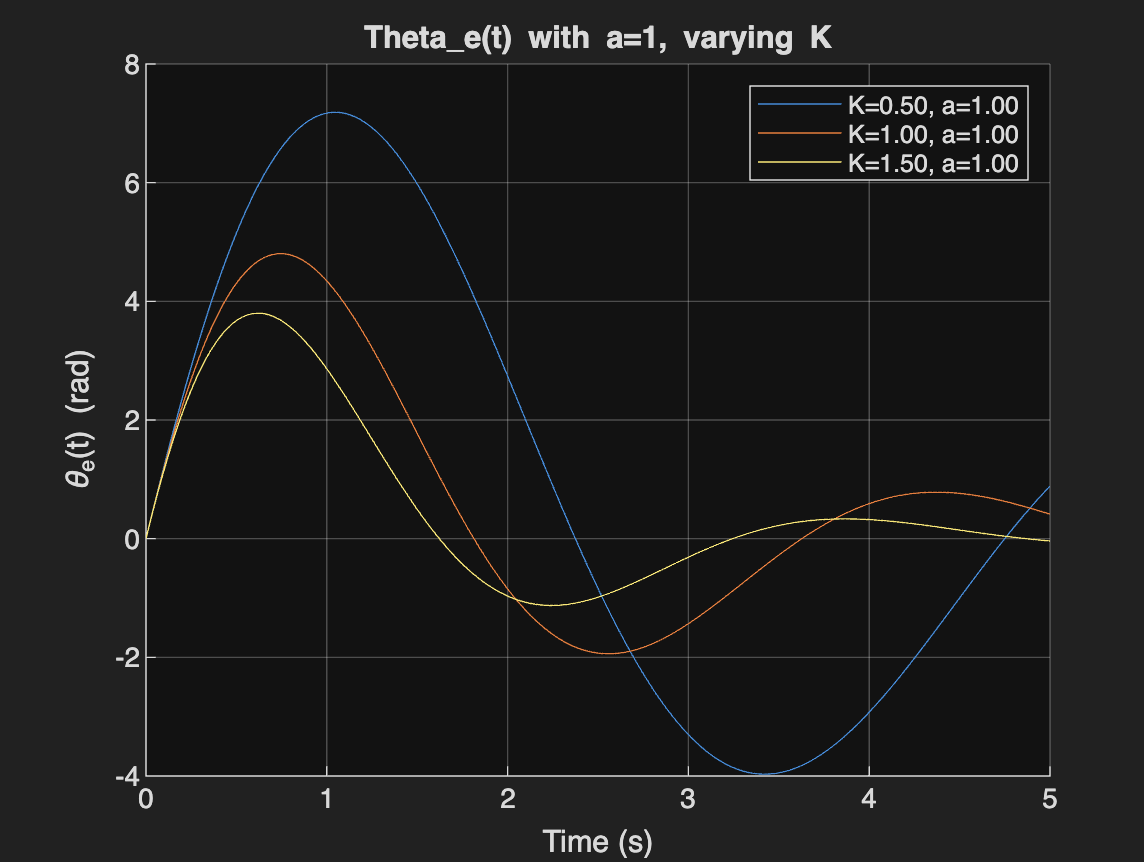
\includegraphics[width=0.6\linewidth]{a=1.png}%
  }{%
    \fbox{\parbox{0.8\linewidth}{a=1.png not found at build time.}}%
  }
  \caption{$\theta_e(t)$ with $a=1$ and varying $K$.}
  \label{fig:varyK}
\end{figure}
\begin{figure}[H]
  \centering
  \IfFileExists{k=1.png}{%
    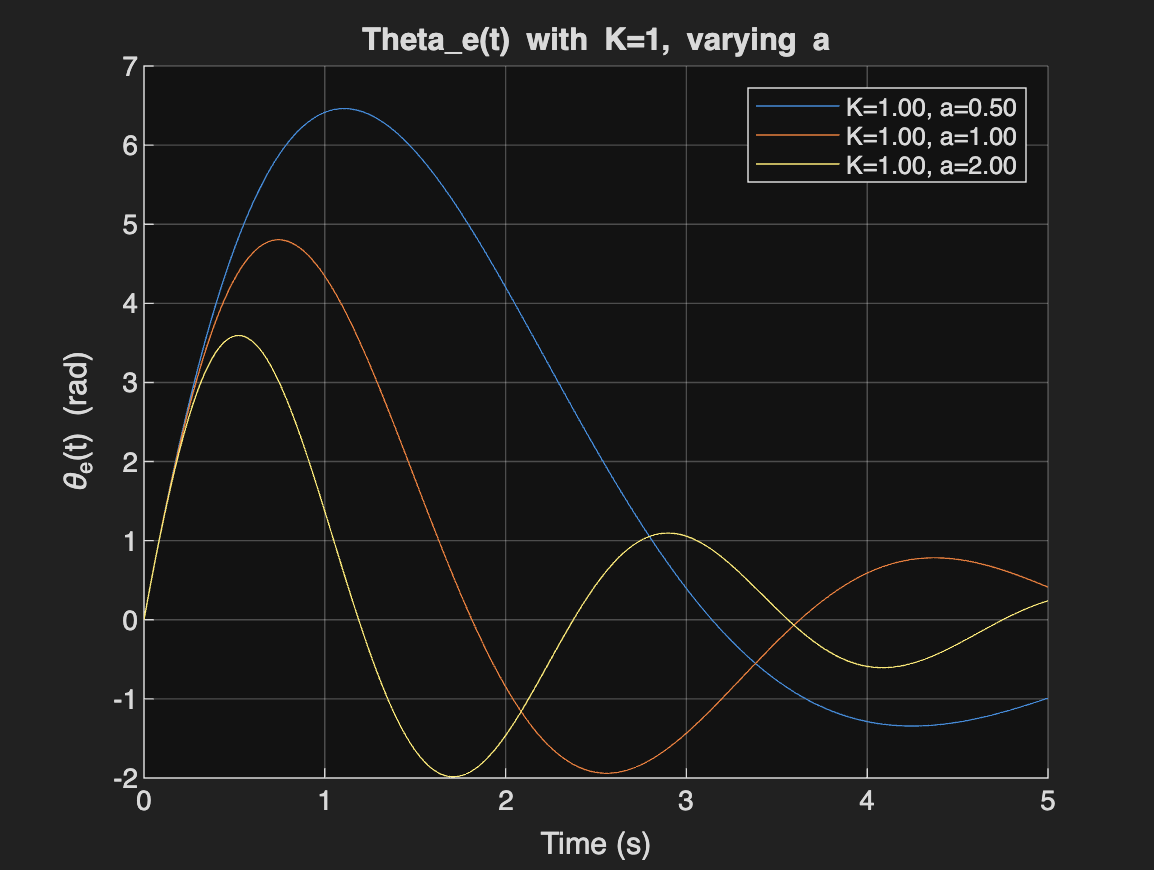
\includegraphics[width=0.6\linewidth]{k=1.png}%
  }{%
    \fbox{\parbox{0.8\linewidth}{k=1.png not found at build time.}}%
  }
  \caption{$\theta_e(t)$ with $K=1$ and varying $a$.}
  \label{fig:varyA}
\end{figure}
\FloatBarrier

\newpage
\section{Discussion Points}
Use the plotted curves (and printed metrics, if enabled) to answer the lab questions:
\begin{itemize}[leftmargin=1.5em]
  \item \textbf{Peak value:} For the chosen sets, higher $K$ (with $a$ fixed) generally lowers the peak because the higher damping suppresses overshoot. Changing $a$ while holding $K$ fixed shifts the frequency more than the peak amplitude.
  \item \textbf{Speed to converge:} The decay envelope is $e^{-Kt/2}$, so larger $K$ visibly shortens settling time. Varying $a$ at fixed $K$ has minor effect on decay rate; the exponent is unchanged.
  \item \textbf{Oscillation frequency:} $\omega_d=\sqrt{4Ka-K^2}$; increasing $a$ increases $\omega_d$ (tighter spacing between zero crossings and peaks). Increasing $K$ slightly reduces $\omega_d$ for constant $a$ because of the $-K^2$ term.
  \item \textbf{Stability boundary:} If $4Ka-K^2\le 0$, the system loses its oscillatory response (critically damped or unstable). All plotted cases stay in the underdamped region.
\end{itemize}



\end{document}
